%% 
%% Copyright 2019 Elsevier Ltd
%% 
%% This file is part of the 'CAS Bundle'.
%% --------------------------------------
%% 
%% It may be distributed under the conditions of the LaTeX Project Public
%% License, either version 1.2 of this license or (at your option) any
%% later version.  The latest version of this license is in
%%    http://www.latex-project.org/lppl.txt
%% and version 1.2 or later is part of all distributions of LaTeX
%% version 1999/12/01 or later.
%% 
%% The list of all files belonging to the 'CAS Bundle' is
%% given in the file `manifest.txt'.
%% 
%% Template article for cas-dc documentclass for 
%% double column output.

%\documentclass[a4paper,fleqn,longmktitle]{cas-dc}
\documentclass[a4paper,fleqn]{cas-dc}

%\usepackage[authoryear,longnamesfirst]{natbib}
%\usepackage[authoryear]{natbib}
\usepackage[numbers]{natbib}
\usepackage{nicefrac}

%%%Author definitions
\def\tsc#1{\csdef{#1}{\textsc{\lowercase{#1}}\xspace}}
\tsc{WGM}
\tsc{QE}
\tsc{EP}
\tsc{PMS}
\tsc{BEC}
\tsc{DE}
%%%

\begin{document}
\let\WriteBookmarks\relax
\def\floatpagepagefraction{1}
\def\textpagefraction{.001}
\shorttitle{Similarity laws of the fiber-matrix interface crack in polymer composites}
\shortauthors{Luca Di Stasio et~al.}

\title [mode = title]{Similarity laws of the fiber-matrix interface crack in polymer composites}                      
%\tnotemark[1,2]

%\tnotetext[1]{This document is the results of the research
   %project funded by the National Science Foundation.}

%\tnotetext[2]{The second title footnote which is a longer text matter
   %to fill through the whole text width and overflow into
   %another line in the footnotes area of the first page.}



\author[1,2]{Luca {Di Stasio}}%[type=editor,
                        %auid=000,bioid=1,
                        %prefix=Sir,
                        %role=Researcher,
                        %orcid=0000-0001-7511-2910]
%\cormark[1]
%\fnmark[1]
%\ead{cvr_1@tug.org.in}
%\ead[url]{www.cvr.cc, cvr@sayahna.org}

%\credit{Conceptualization of this study, Methodology, Software}

\author[1]{Janis Varna}

\author[2]{Zoubir Ayadi}

%\fnmark[2]
%\ead{cvr3@sayahna.org}
%\ead[URL]{www.sayahna.org}

%\credit{Data curation, Writing - Original draft preparation}

\address[1]{Lule\aa\ University of Technology, University Campus, SE-97187 Lule\aa, Sweden}

\address[2]{Universit\'e de Lorraine, EEIGM, IJL, 6 Rue Bastien Lepage, F-54010 Nancy, France}

%\author%
%[1,3]
%{Rishi T.}
%\cormark[2]
%\fnmark[1,3]
%\ead{rishi@stmdocs.in}
%\ead[URL]{www.stmdocs.in}
%
%\address[3]{STM Document Engineering Pvt Ltd., Mepukada,
%    Malayinkil, Trivandrum 695571, India}
%
%\cortext[cor1]{Corresponding author}
%\cortext[cor2]{Principal corresponding author}
%\fntext[fn1]{This is the first author footnote. but is common to third
%  author as well.}
%\fntext[fn2]{Another author footnote, this is a very long footnote and
%  it should be a really long footnote. But this footnote is not yet
%  sufficiently long enough to make two lines of footnote text.}
%
%\nonumnote{This note has no numbers. In this work we demonstrate $a_b$
%  the formation Y\_1 of a new type of polariton on the interface
%  between a cuprous oxide slab and a polystyrene micro-sphere placed
%  on the slab.
%  }

\begin{abstract}
This template helps you to create a properly formatted \LaTeX\ manuscript.

\noindent\texttt{\textbackslash begin{abstract}} \dots 
\texttt{\textbackslash end{abstract}} and
\verb+\begin{keyword}+ \verb+...+ \verb+\end{keyword}+ 
which
contain the abstract and keywords respectively. 

\noindent Each keyword shall be separated by a \verb+\sep+ command.
\end{abstract}

%\begin{graphicalabstract}
%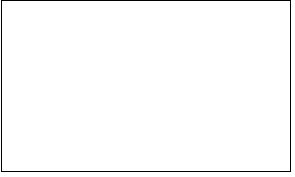
\includegraphics{figs/grabs.pdf}
%\end{graphicalabstract}
%
%\begin{highlights}
%\item Research highlights item 1
%\item Research highlights item 2
%\item Research highlights item 3
%\end{highlights}

\begin{keywords}
Fiber Reinforced Polymer Composite (FRPC) \sep Debonding \sep Similarity \sep Dimensional analysis
\end{keywords}


\maketitle

\section{Introduction}

One of the most promising developments in Fiber Reinforced Polymer Composites (FRPCs) for advanced structural applications is currently represented by \emph{thin-ply} laminates~\cite{Kopp2017}. Constituted by extremely thin plies, with $t_{90^{\circ}}$ as small as just $\sim4-5$ fiber diameters, this family of laminates is characterized by its damage tolerance, in particular the capability of delaying to higher strains and even suppressing the onset and propagation of transverse cracks~\cite{Cugnoni2018}. The recent experimental assessment of transverse cracks suppression in \emph{thin-ply} laminates~\cite{Sasayama2003,Saito2012,Amacher2014} validates the existence of a \emph{ply-thickness} effect~\cite{Amacher2014} at scales $10x$ smaller than those at which it was originally observed at the end of the 1970's~\cite{Bailey1979}.\\
Onset of transverse cracks coincides at the microscopic level with the formation of fiber/matrix interface cracks~\cite{Bailey1981}, or debonds. After the inter-fiber stress~\cite{Asp1996} and strain concentration~\cite{Kies1962} causes the matrix to fail at or close the fiber interface, debonds grow along the fiber arc direction until a maximum or critical size is reached. If the applied load is increased, debonds move into the matrix or ``kink'' out of the fiber/matrix interface~\cite{Zhang1997,Paris2007}. Coalescence of debonds then occurs, which corresponds macroscopically to through-the-thickness transverse crack propagation~\cite{Zhang1997,Zhuang2018}. Finally, propagation through the specimen width occurs~\cite{Zhang1997}.\\
Given that \emph{thin-plies}, as previously noted, can reach nowadays thicknesses of just $\sim4-5$ fiber diameters, the characteristic size of the ply, i.e. the thickness $t_{90^{\circ}}$, is now comparable in magnitude to the characteristic size of debonds, i.e. the fiber diameter $2R_{f}$, such that $\nicefrac{t_{90^{\circ}}}{\left(2R_{f}\right)}\sim\mathcal{O}\left(1\right)$. This has motivated in recent years a renewed interest in debond growth modeling~\cite{Zhuang2018,Sandino2016,Varna2017,Sandino2018}. Since the elastic solution to the interface crack problem implies an oscillating solution at the crack tip~\cite{Comninou1977} in the \emph{open} case (crack faces not in contact), Stress Intensify Factors (SIFs) are not defined and debond growth characterization has focused on the determination of Mode I, Mode II and total Energy Release Rate (ERR). Many authors have reported their results in normalized form~\cite{Paris2007,Toya1974,Paris1996}, by defining a reference ERR $G_{0}$. The definition of such reference ERR would be useful to establish similarity laws and thus to allow comparisons between different material systems, scales, loads and microstructural arrangement. However, no agreement can be found in the literature on the very definition of $G_{0}$ and expressions vary between authors. Furthermore, no clear derivation of $G_{0}$ has been proposed. In this brief contribution, we provide a derivation of $G_{0}$ based on arguments of dimensional analysis, material homogenization and fracture mechanics; we then apply the derived expression of reference ERR to the analysis of debond growth in Representative Volume Elements (RVEs) of UD composites and cross-ply laminates. 

\section{Dimensional analysis}

We first recall that the Energy Release Rate $G$ has units of energy $E$ per unit area:

\begin{equation}\label{eq:errunits}
\left[G\right]=\frac{E}{L^{2}},
\end{equation}

where $L$ stands for unit of length. By algebraic manipulation of Equation~\ref{eq:errunits} we can write the units of ERR as

\begin{equation}\label{eq:errunitsreworked}
\frac{E}{L^{2}}=\frac{F\cdot L}{L^{2}}=\frac{F}{L^{2}}\frac{L}{L}L,
\end{equation}

where $F$ stands for unit of force. We recognize that, in Equation~\ref{eq:errunitsreworked}

\begin{equation}\label{eq:sigmaepsunits}
\frac{F}{L^{2}}=\left[\sigma\right]\qquad\frac{L}{L}=\left[\varepsilon\right],
\end{equation}

where $\sigma$ and $\varepsilon$ are respectively stress and strain. The Energy Release Rate is thus dimensionally equivalent to a reference stress $\sigma_{ref}$ times a reference strain $\varepsilon_{ref}$ times a refence length $l_{ref}$ and we can write

\begin{equation}\label{eq:G}
G\sim\sigma_{ref}\varepsilon_{ref}l_{ref}.
\end{equation}

In the case of uniaxial loading, we can assume that: in a stress-controlled experiment, $\sigma_{ref}$ is equal to the applied stress $\sigma_{0}$ and $\varepsilon_{ref}$ to the average strain $\varepsilon_{0}$ in the Representative Volume Element (RVE); in a strain-controlled experiment, $\varepsilon_{ref}$ is equal to the applied strain $\varepsilon_{0}$ and $\sigma_{ref}$ to the average stress $\sigma_{av}$ in the Representative Volume Element (RVE).\\
Under the assumption of linear elastic material constituents, we have, respectively for a stress- and strain-controlled experiment:

\begin{equation}\label{eq:elasticresponse}
\varepsilon_{av}=E_{homo}\sigma_{0}\qquad\sigma_{av}=E_{homo}\varepsilon_{0},
\end{equation}

where $E_{homo}$ is a homogenized RVE Young's modulus which measures the RVE elastic response in the presence of different material phases and damage. It is worth to point out here that, as we are interested in studying debond growth in the context of transverse crack onset, RVEs are loaded in the direction transverse to the fibers in the layer where debonds are present. Furthermore, we consider RVEs that are 2-dimensional and under the assumption of plane strain or plane stress conditions. This implies, considering the elastic response of a transversely isotropic material in its plane of transverse isotropy (indeces $2-3$, index $1$ corresponds to the axis of rotational symmetry) with no damage, that~\cite{Timoshenko1987,Mantic2009}

\begin{equation}\label{eq:elasticresponse}
E_{homo}=\frac{E_{2}}{1-\nu_{12}\nu_{21}}\qquad E_{homo}=E_{2},
\end{equation}

respectively for plane strain and plane stress.
\section{Representative Volume Elements (RVEs)}






\section{Similarity laws}



\section{Conclusions}



%% Loading bibliography style file
\bibliographystyle{model1-num-names}
%\bibliographystyle{cas-model2-names}

% Loading bibliography database
\bibliography{refs}


%\vskip3pt

%\bio{}
%Author biography without author photo.
%Author biography. Author biography. Author biography.
%Author biography. Author biography. Author biography.
%Author biography. Author biography. Author biography.
%Author biography. Author biography. Author biography.
%Author biography. Author biography. Author biography.
%Author biography. Author biography. Author biography.
%Author biography. Author biography. Author biography.
%Author biography. Author biography. Author biography.
%Author biography. Author biography. Author biography.
%\endbio
%
%\bio{figs/pic1}
%Author biography with author photo.
%Author biography. Author biography. Author biography.
%Author biography. Author biography. Author biography.
%Author biography. Author biography. Author biography.
%Author biography. Author biography. Author biography.
%Author biography. Author biography. Author biography.
%Author biography. Author biography. Author biography.
%Author biography. Author biography. Author biography.
%Author biography. Author biography. Author biography.
%Author biography. Author biography. Author biography.
%\endbio
%
%\bio{figs/pic1}
%Author biography with author photo.
%Author biography. Author biography. Author biography.
%Author biography. Author biography. Author biography.
%Author biography. Author biography. Author biography.
%Author biography. Author biography. Author biography.
%\endbio

\end{document}

